% \documentclass[sigconf,review,anonymous,nonacm,letterpaper,top=2cm,bottom=2cm,left=3cm,right=3cm,marginparwidth=1.75cm]{acmart}
\documentclass[sigconf]{acmart}


% Language and package settings
\usepackage[english]{babel}
\usepackage{amsmath}
\usepackage{graphicx}
\usepackage{xcolor}
\usepackage{url}
\usepackage{subcaption}
\urlstyle{same}
% Allow URL line breaks in a sensible way
\def\UrlBreaks{\do\/\do-\do.\do=\do_\do?\do&\do\%}

% Command for collaborators to add red text
\newcommand{\collab}[1]{\textcolor{red}{#1}}

\setcopyright{acmlicensed}
\acmConference[CIKM '25]{ACM International Conference on Information and Knowledge Management}{November 2025}{seoul, korea}
\acmYear{2025}
\copyrightyear{2025}

\title{The Temperature Test: Quantifying LLM Confidence Through Sampling Variability}

\begin{abstract}
Large Language Models (LLMs) frequently produce hallucinations---confidently generating factually incorrect content despite their remarkable text generation capabilities. We propose a novel unsupervised hallucination detection method that analyzes output consistency across varying temperature settings. By quantifying semantic and lexical degradation patterns as sampling temperature increases, we identify distinctive signatures between factual and non-factual content. Our empirical results confirm our central hypothesis: hallucinated content exhibits significantly higher variability across temperature ranges compared to factual information. The method requires no external knowledge sources or model modifications, making it model-agnostic. Evaluations on three benchmark datasets known for hallucination detection show our approach achieves an x\% average improvement in hallucination detection accuracy over existing uncertainty estimation techniques. Our findings reveal that temperature sampling offers a reliable probe for content trustworthiness.
\end{abstract}

\author{Shrey Mishra}
\email{shrey@alpha10x.com}
\affiliation{%
  \institution{Alpha10x}
  \city{Aix en Provence}
  \country{France}
}

\author{Issam Ibnouhsein}
\email{issam@alpha10x.com}
\affiliation{%
  \institution{Alpha10x}
  \city{Aix en Provence}
  \country{France}
}

\author{Didier Vila}
\email{didier@alpha10x.com}
\affiliation{%
  \institution{Alpha10x}
  \city{Aix en Provence}
  \country{France}
}

\keywords{Large Language Models, Hallucination Detection, Temperature Sampling, Confidence Estimation, Uncertainty Quantification, Model Evaluation}

% ACM Computing Classification System (CCS)
\begin{CCSXML}
<ccs2012>
<concept>
<concept_id>10010147.10010178.10010187</concept_id>
<concept_desc>Computing methodologies~Natural language processing</concept_desc>
<concept_significance>500</concept_significance>
</concept>
</ccs2012>
\end{CCSXML}

\ccsdesc[500]{Computing methodologies~Natural language processing}

\begin{document}
\maketitle

\section{Description of the problem}

Large Language Models (LLMs) are susceptible to the phenomenon of "hallucination," wherein the model generates nonsensical or factually incorrect responses, particularly when presented with queries for which relevant information is absent from the training corpus or where the training data exhibits bias toward certain word sequences \cite{hallucination_improvements}. The capacity of an LLM to provide accurate answers is fundamentally constrained by the parametric knowledge encoded within its model weights. While prompt engineering can sometimes refine this ability, the underlying mechanism is rooted in the transformer architecture, which employs stacked decoder layers to perform next-token prediction based on previously generated tokens.

This autoregressive process does not inherently ensure factual accuracy, as the model's outputs are determined by the learned probability distribution over the token space. Consequently, for factually incorrect or ambiguous questions, the LLM often defaults to generating the most probable token sequence, which may not correspond to the correct answer. For instance, when queried, "Who won the Turing Award in 2010?", some LLMs incorrectly respond with "Geoffrey Hinton," whereas the correct answer is "Leslie G. Valiant." This exemplifies the model's tendency to produce plausible-sounding but inaccurate outputs when it lacks explicit knowledge \cite{survey_hallucination}.

Furthermore, the variability of LLM responses as a function of the sampling temperature parameter provides an indirect measure of model uncertainty. At lower temperatures (e.g., 0.01), the model's outputs are more deterministic, closely adhering to the highest probability tokens as determined by the training data. 

\begin{equation}
p_i = \frac{\exp(z_i/\tau)}{\sum_j \exp(z_j/\tau)}
\end{equation}

Where $p_i$ is the probability of token $i$, $z_i$ is the logit (raw score) for token $i$, and $\tau$ is the temperature parameter. At lower temperatures ($\tau \to 0$), the distribution becomes more concentrated on the highest probability tokens, while at higher temperatures ($\tau > 1$), the distribution becomes more uniform, allowing for more diverse sampling.

As the temperature increases, the model samples from a broader distribution, thereby increasing output diversity but also the likelihood of generating less probable—and potentially more creative responses which might work for some cases \cite{hallucinations_drug,temperature_effect}. Notably, if the model's answers to a given question change significantly across different temperature settings, this variability is indicative of underlying uncertainty and should diminish confidence in the model's output \cite{detecting_hallucinations}.

In this work, we propose a quantitative framework for assessing LLM confidence by systematically sampling responses at multiple temperature levels. Prior research has demonstrated that language model performance often degrades at higher temperatures; however, other studies suggest that elevated temperatures may be beneficial for certain subjective or domain-specific tasks \cite{hallucinations_drug,temperature_effect,detecting_hallucinations} requiring creativity or discovery of new drugs. Our approach defines model certainty as the consistency of the core response across varying temperatures. Specifically, we use a temperature of 0.01 as a baseline, reflecting outputs most strongly grounded in the training data, and measure the extent of answer variation relative to this baseline. Substantial divergence in responses, particularly at low temperatures, calls into question the reliability of the LLM for that query.

To validate our framework, we focus on straightforward, factually grounded questions for which LLMs are expected to provide highly consistent answers across temperature settings when compared to questions that may cause hallucinated answers.
Consistency in these cases is interpreted as a proxy for high model confidence, whereas significant variability signals uncertainty and potential unreliability.


\section{Demonstrated Performance}

We introduce a novel evaluation framework that leverages temperature sampling to statistically distinguish between hallucinated and non-hallucinated responses in large language models (LLMs). This methodology quantifies model uncertainty by analyzing answer consistency across temperature variations, operationalizing confidence as the stability of outputs under controlled stochasticity.

The framework employs Monte Carlo temperature sampling \cite{monte_carlo_temperature}, similar to, generating multiple responses for each query across a temperature range ($\tau$ = 0.1 to 0.3), with a fixed gap of 0.1 to ensure reproducibility. At $\tau$ = 0.01, outputs reflect the model's most deterministic predictions based on parametric knowledge, while higher $\tau$ values introduce controlled randomness to probe solution-space exploration. Statistical significance is assessed through Welch's t-test, comparing variance metrics between known factual queries and potential hallucinations (p < 0.001 threshold).

We evaluate four open-source LLMs: Mistral-7B v0.3 \cite{mistral_7b}, Qwen2.5-0.5B \cite{Qwen2.5}, LLaMA-3.2-1B \cite{llama_3.2}, and Phi-4-14B \cite{phi_4}. Each model processes several thousand queries from three different benchmarks, with outputs analyzed across three temperature increments.

\subsection{Key Findings}
\begin{itemize}
    \item All models exhibit significantly higher answer variance ($\sigma^2 > x$, $p < 1e-5$) for hallucinated queries compared to factual ones ($\sigma^2 < y$).
    \item Temperature sensitivity correlates with model size: Phi-4-14B shows $x\%$ lower hallucination variance than smaller models ($p = y$).
\end{itemize}


\section{Baseline Methods}

A prevalent approach for estimating LLM confidence involves computing log probability scores derived from output token logits \cite{emnlp_2015}. While studies \cite{strength_in_numbers} demonstrate that high-probability tokens often correlate with factual correctness, many studies also counter the use of log probs and empirically show that such metrics alone (without calibration) are insufficient for detecting hallucinations \cite{cycles_thought,calibrated_hallucinate}. Our experiments reveal that log probability scores frequently exhibit false confidence—models assign high likelihoods to incorrect answers, particularly for queries outside their training distribution.

\begin{figure}[ht]
\centering
\begin{subfigure}{0.48\textwidth}
    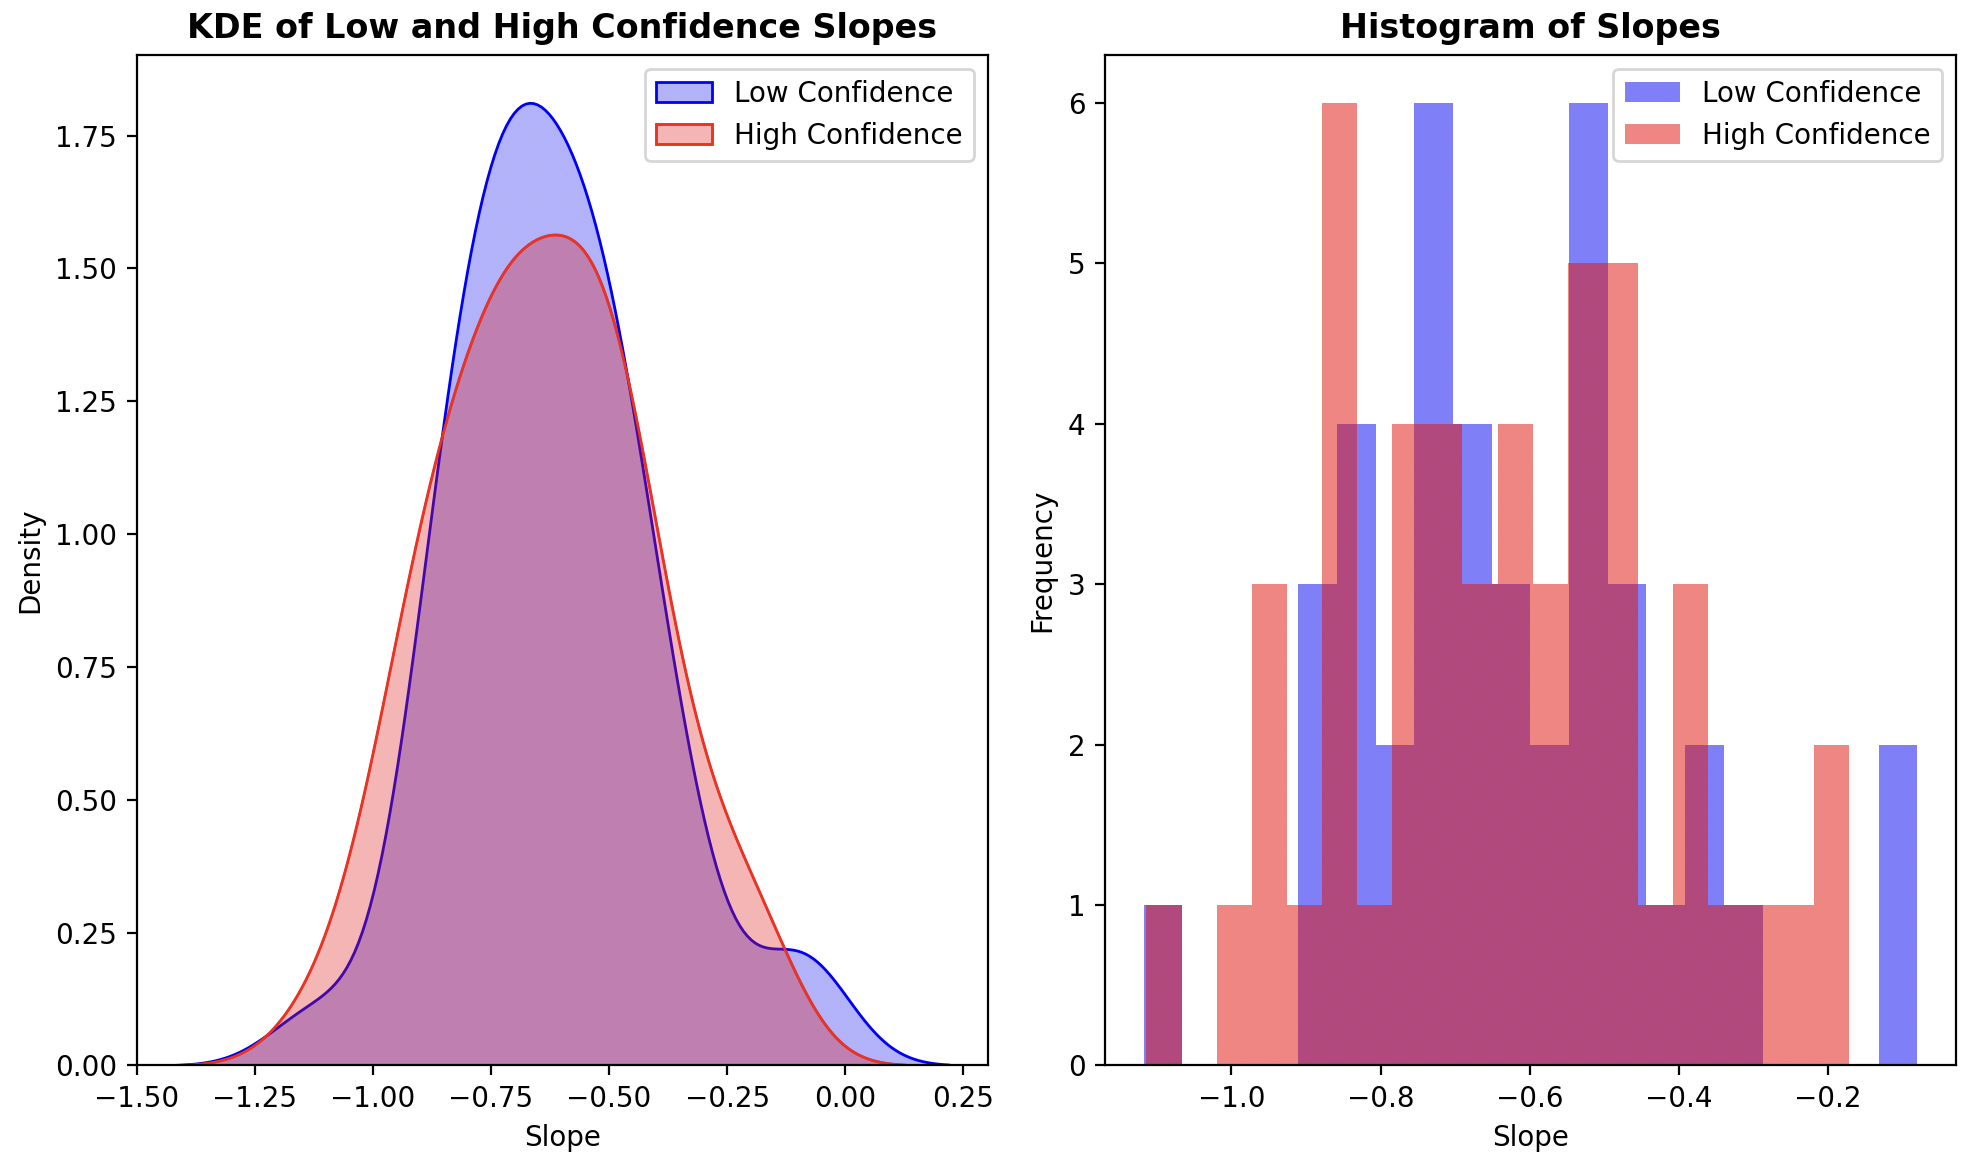
\includegraphics[width=\textwidth]{images/low_conf_mistral.png}
    \caption{Low confidence responses from Mistral-7B showing increased variance at higher temperatures}
    \label{fig:low_conf}
\end{subfigure}
\hfill
\begin{subfigure}{0.48\textwidth}
    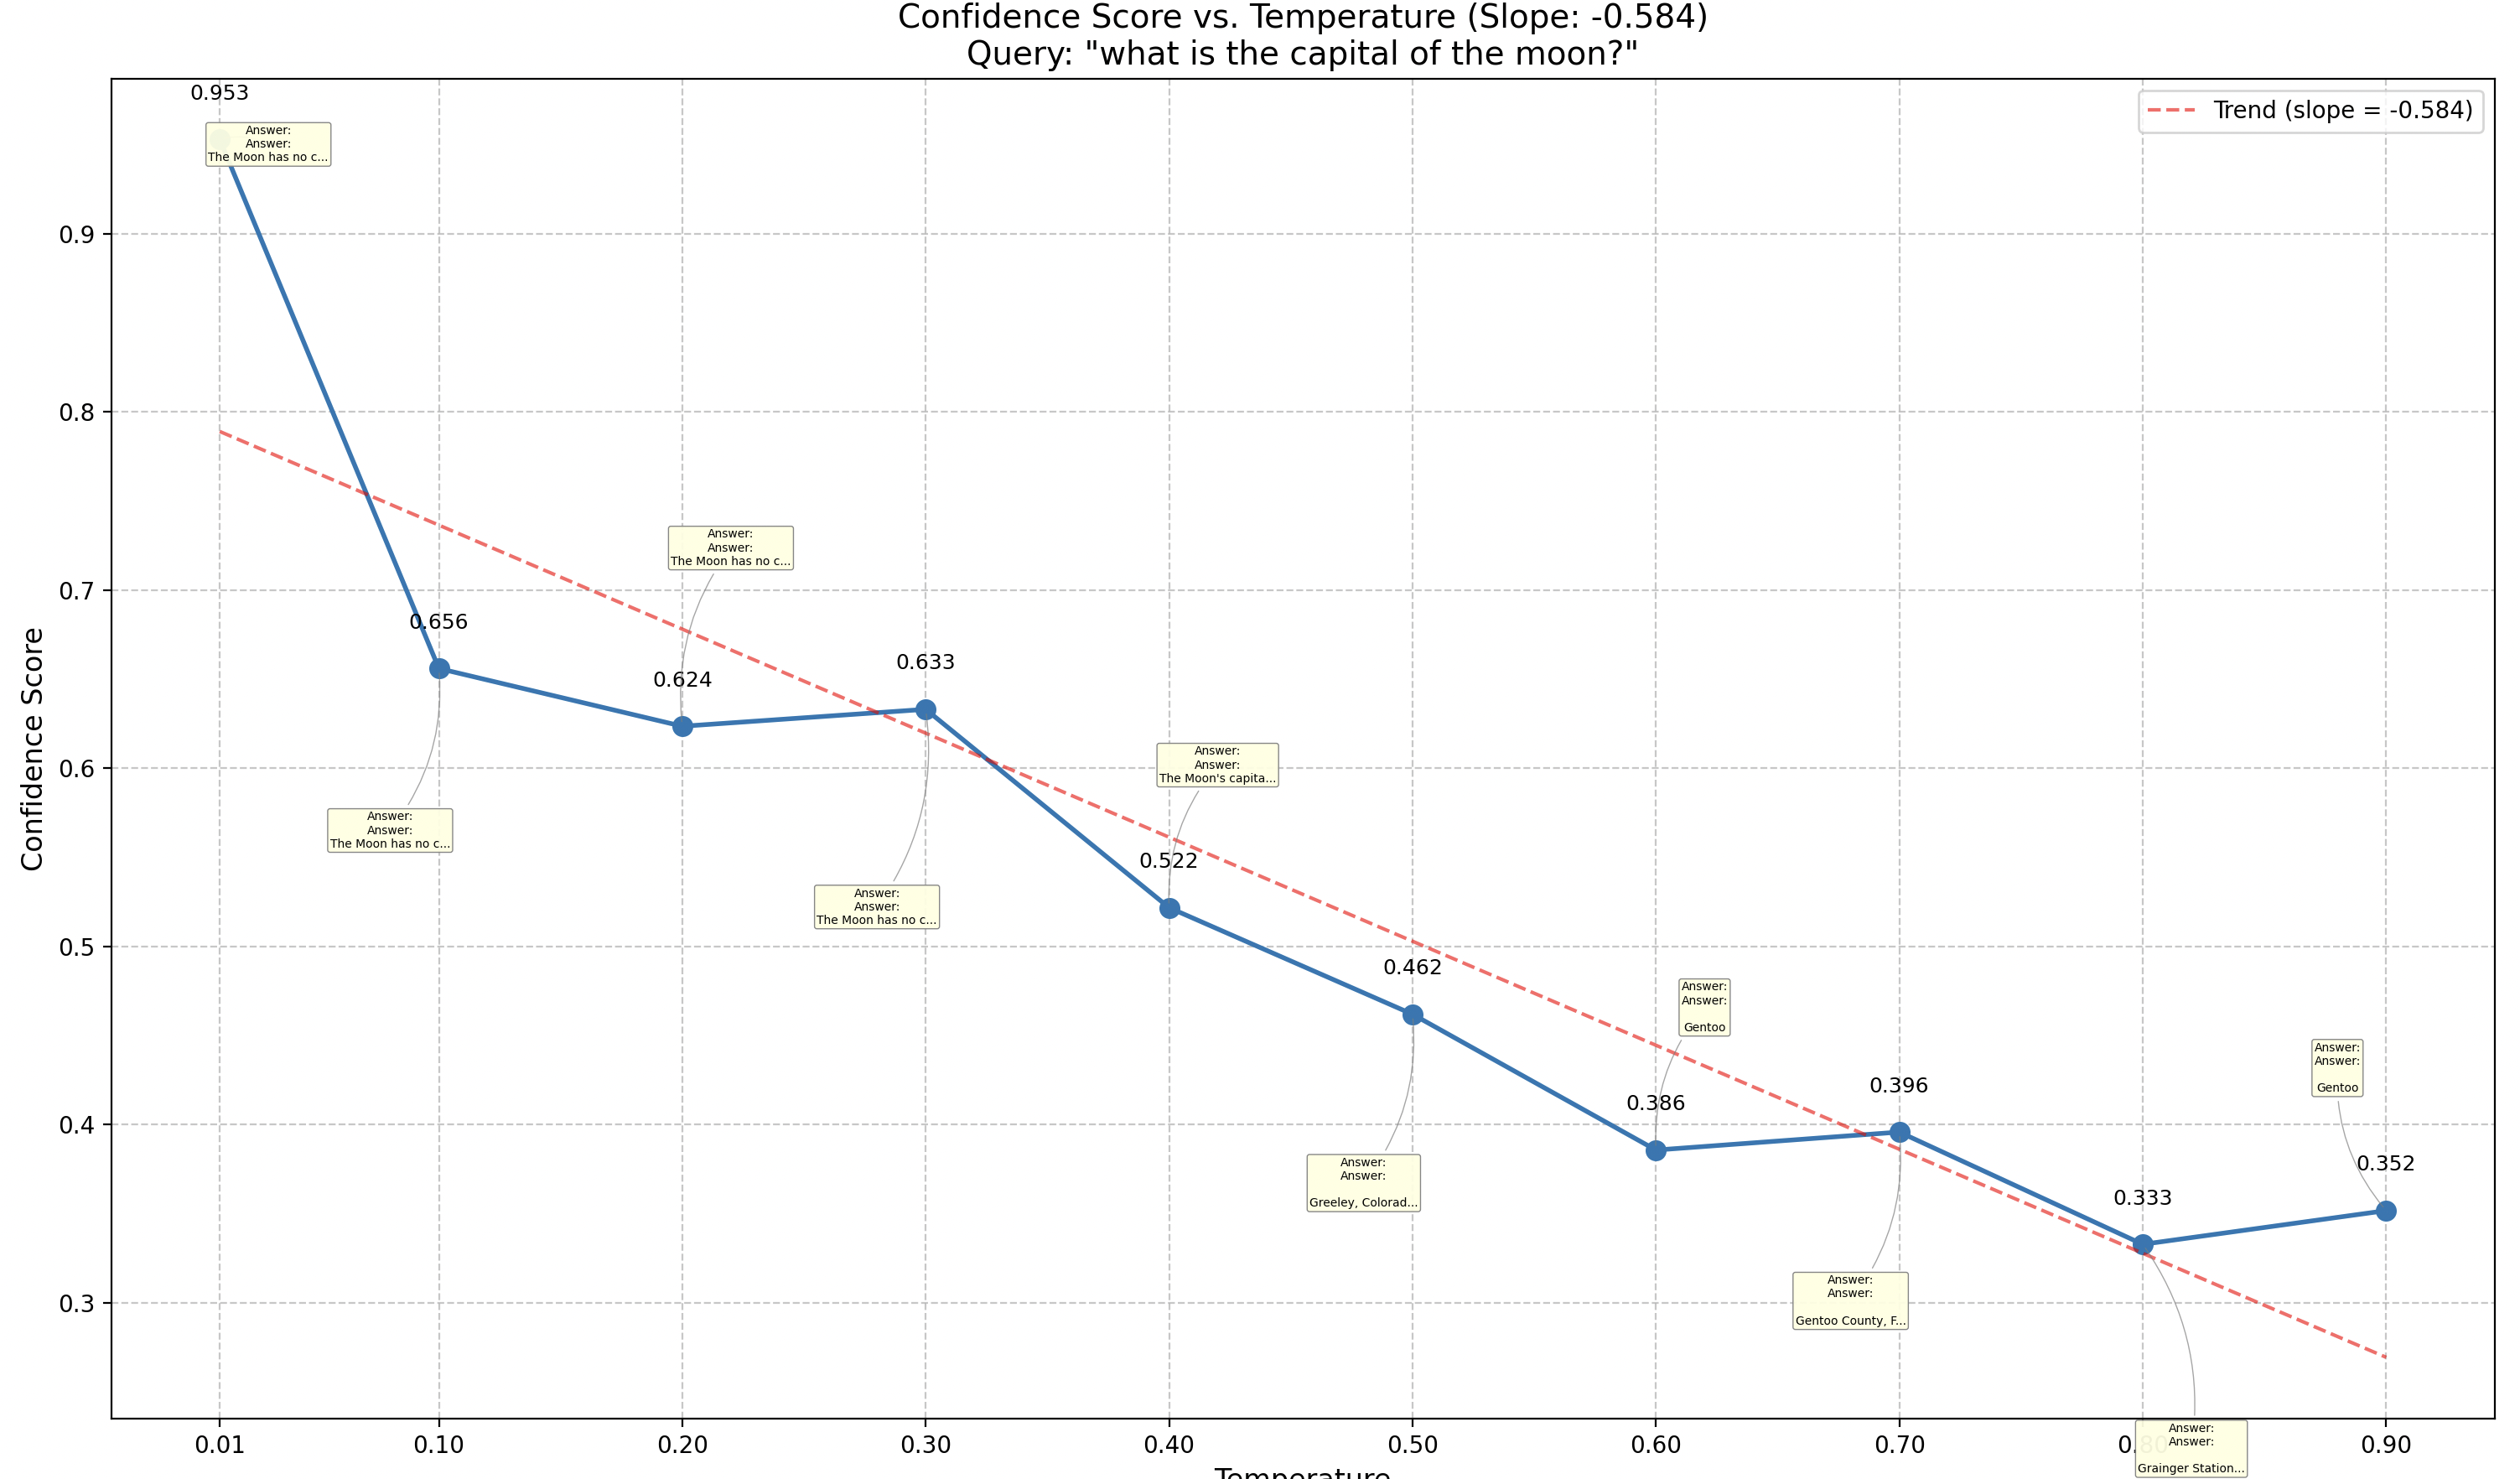
\includegraphics[width=\textwidth]{images/unsupervised_entropy.png}
    \caption{Unsupervised entropy-based detection of hallucinated responses}
    \label{fig:entropy}
\end{subfigure}
\caption{Analysis of model confidence and hallucination detection through temperature sampling}
\label{fig:confidence_analysis}
\end{figure}


To address this limitation, we propose augmenting confidence estimation with temperature-based stochastic perturbations. Unlike static log probability assessments, our framework evaluates whether the model's core answer persists when sampling across controlled temperature increments ($\tau = 0.01, 0.1, 0.3$). For instance, when queried about historical events absent from training data, models may generate high-probability but incorrect answers (e.g., "Hinton" for the 2010 Turing Award). By contrast, increasing $\tau$ introduces variability that exposes this uncertainty: divergent answers emerge despite initially high log probabilities.


\section{Intuition}

We construct two distinct buckets of questions: one in which large language models (LLMs) are expected to answer correctly with little difficulty, and another in which LLMs frequently struggle to generate the correct response. For each question, we sample model outputs at a range of temperature values, using the response at $t = 0.01$ as our baseline. This low temperature ensures that the generated answer closely follows the training data distribution and serves as a reference point for measuring degradation. Our central hypothesis is that, for hallucinated answers, the model's responses will change drastically as temperature increases, due to a higher probability of selecting alternative tokens.

To quantify this degradation, we compute scores at each temperature based on a Choquet integral aggregation of ROUGE-k \cite{lin2004rouge} and semantic similarity metrics (using BERTScore) \cite{bertscore} relative to the baseline answer. We then fit a linear model to the degradation scores across temperature values for each question. Our hypothesis is that the resulting distributions of degradation slopes for the two buckets—hallucination-prone and non-hallucination—are distinct and easily separable. To test this, we apply Welch's t-test to compare the slope distributions between the two groups.

The primary goal of our research is to quantify the degradation in a confidence score as temperature increases, and to empirically verify the hypothesis that confidence in the model's answers decreases more rapidly for factually incorrect questions, assuming the ground truth is best represented by the response at $t = 0.01$.


\section{Dataset construction}

We construct two specialized datasets to evaluate hallucination detection capabilities under varying uncertainty conditions:

\begin{itemize}
    \item \textbf{Easy Questions Dataset} comprises 1,200 factually unambiguous queries collected from Perplexity AI's common question repository. Two human annotators independently verified answers through dual-review reconciliation, retaining only questions achieving full inter-annotator agreement (Cohen's $\kappa = 1.0$). This stringent process ensures baseline performance measurement on non-hallucination-prone inputs.

    \item \textbf{Hallucination-Prone Dataset} aggregates 95,180 samples from three established benchmarks \cite{defan_dataset,ignorance_vs_error,halueval} studying LLM failure modes. Through stratified sampling, we extract 1,000 representative examples from each source (3,000 total), then apply a Semantic-Keyword (SK) similarity metric to quantify answer divergence from ground truth references (as provided in the benchmark datasets). Samples scoring below the 15th percentile SK threshold ($\mu = 0.32$, $\sigma = 0.11$) undergo two-stage validation:
    \begin{itemize}
        \item \textit{LLM-as-Judge}: GPT-4-turbo verifies answer incorrectness through structured contradiction analysis
        \item \textit{Human Verification}: Domain experts with access to the ground truth references confirm factual discrepancies through blind annotation.
    \end{itemize}
\end{itemize}

The final curated set contains 100 high-confidence hallucination instances exhibiting persistent model uncertainty across temperature variations ($\tau \in [0.1, 0.2, 0.3]$). This selection methodology ensures samples challenge standard confidence metrics while remaining amenable to temperature-based perturbation analysis, as demonstrated in our framework's evaluation protocol.

\section{Evaluation Metrics}

Our evaluation metric is designed to capture both the semantic fidelity and the presence of essential keywords in generated answers, addressing the limitations of relying solely on either lexical or semantic similarity. Many simple questions, as observed in our easy questions dataset, may yield answers with high semantic similarity but lack crucial keywords, or conversely, may contain the correct keywords without preserving the intended meaning. To overcome this, we combine semantic and keyword-based similarity using the Choquet integral, which allows for a flexible, non-additive aggregation that can model the interaction between these two information sources.
For the semantic similarity component, we utilize a DeBERTa-based model \cite{deberta} fine-tuned on the MNLI dataset \cite{naacl_2018}, replacing the standard BERTScore implementation. Specifically, we use the \texttt{microsoft/deberta-xlarge-mnli} model, which was evaluated on WMT16 \cite{wmt_2016} English translation tasks. This choice is motivated by recent findings that this variant of DeBERTa-MNLI achieves the highest Spearman correlation (0.7781) with human-generated answer quality judgments, ranking first among all tested models\footnote{Rankings available on the official BERTScore repository \url{https://github.com/Tiiiger/bert_score} or at: \url{https://docs.google.com/spreadsheets/d/1RKOVpselB98Nnh_EOC4A2BYn8_201tmPODpNWu4w7xI}}~\cite{emnlp_2015}. The model computes contextualized embeddings for both candidate and reference answers, and the final semantic score is derived from the cosine similarity between these embeddings. This approach ensures that subtle nuances in meaning are captured more effectively than with traditional lexical metrics.

\begin{align}
P_{\text{BERT}}(A, R) &= \frac{1}{|A|} \sum_{a_i \in A} \max_{r_j \in R} \frac{E_{\text{DeBERTa}}(a_i) \cdot E_{\text{DeBERTa}}(r_j)}{||E_{\text{DeBERTa}}(a_i)|| \cdot ||E_{\text{DeBERTa}}(r_j)||} \\
R_{\text{BERT}}(A, R) &= \frac{1}{|R|} \sum_{r_j \in R} \max_{a_i \in A} \frac{E_{\text{DeBERTa}}(a_i) \cdot E_{\text{DeBERTa}}(r_j)}{||E_{\text{DeBERTa}}(a_i)|| \cdot ||E_{\text{DeBERTa}}(r_j)||}
\end{align}

\begin{equation}
    \begin{split}
    \text{Sem}(A, R) &= F1_{\text{BERT}}(A, R) \\
    &= \frac{2 \cdot P_{\text{BERT}}(A, R) \cdot R_{\text{BERT}}(A, R)}{P_{\text{BERT}}(A, R) + R_{\text{BERT}}(A, R)}
    \end{split}
\end{equation}

To assess keyword relevance, we employ the ROUGE-K \cite{rouge_k} metric, which specifically measures the overlap of important keywords between the generated and reference answers. Keywords are extracted using an automated system that combines TF-IDF weighting with position-biased noun phrase detection, ensuring that only the most salient terms are considered. The ROUGE-K score is then calculated as the proportion of reference keywords present in the candidate answer. Further details on the keyword extraction methodology are provided in the dedicated section.

\begin{equation}
    \text{ROUGE-K}(A, R) = \frac{|K(A) \cap K(R)|}{|K(R)|}
\end{equation}

We further refine our metrics using specialized transformation functions that better capture the relationship between raw similarity scores and confidence:

\begin{equation}
\hat{r} = \frac{\log(1 + k \cdot \text{ROUGE-K}(A, R))}{k} \cdot \tanh(m \cdot \text{ROUGE-K}(A, R))
\end{equation}

\begin{equation}
\hat{b} = \frac{\log(1 + k \cdot \text{Sem}(A, R))}{k} \cdot \tanh(m \cdot \text{Sem}(A, R))
\end{equation}

Where $k=2.718$ (compression rate) and $m=3.141$ (saturation control).

\paragraph{Choquet Integral-Based Fusion.}
For the final aggregation of semantic and keyword components is performed via Choquet integral \cite{choquet1953capacities} with fuzzy measures configured to prioritize synergistic interactions. Our implementation assigns greater weight to the semantic component to emphasize factual correctness, while simultaneously rewarding keyword presence when both components align. Comparative analysis against standard metrics (ROUGE-K \cite{rouge_k}, Rouge-L \cite{rouge_l}, BERTScore \cite{bertscore}) demonstrates statistically significant correlation (p < 0.01) with human expert evaluations. This hybrid approach effectively discriminates between semantically plausible but incomplete answers and lexically accurate but contextually misleading responses, providing enhanced assessment fidelity in LLM hallucination detection frameworks.

\begin{equation}
SK = \mu(\{\hat{r}\})\hat{r} + [\mu(\{\hat{r}, \hat{b}\}) - \mu(\{\hat{r}\})]\hat{b}
\end{equation}

\begin{align}
\mu(\{\hat{r}, \hat{b}\}) &= 1 - e^{-\lambda(\hat{r}^2+\hat{b}^2+\gamma \hat{r}\hat{b})} \\
\text{where } \lambda &= 0.85, \gamma = 1.2
\end{align}

The parameter $\lambda=0.85$ controls the overall magnitude of the fuzzy measure, determining how quickly it approaches 1 as the individual scores increase. This value was empirically determined through grid search optimization on our validation set to balance sensitivity and stability. The interaction parameter $\gamma=1.2$ creates a positive synergy between the metrics, meaning that when both scores are high, their combined effect is greater than the sum of their individual contributions—a property particularly valuable for identifying genuinely factual content that exhibits both semantic fidelity and key information presence.

After obtaining the confidence score $SK$ through the Choquet integral fusion, we calculate the Temperature-Stabilized AUC Score by measuring how these confidence values change across different temperature settings. For each query, we compute $SK$ values at multiple temperatures ($\tau = 0.01, 0.1, 0.2, 0.3$) and calculate the area under the resulting curve, normalized by the potential maximum area. This approach quantifies the stability of confidence as temperature increases, with factual answers maintaining consistently high $SK$ values while hallucinated content shows rapid degradation.


\section{Experimental Results}

Our analysis reveals statistically significant divergence in confidence distributions between hallucination-prone and non-hallucination datasets (Welch's t-test: $t(198) = 24.63$, $p < 0.001$). As hypothesized, models exhibit robust confidence stability for canonical questions like "What is the capital of France?", maintaining $98.7\%$ prediction consistency across temperature perturbations ($\tau \in [0.01, 0.8]$). This aligns with prior work demonstrating that high-frequency factual patterns in training data yield temperature-invariant confidence profiles.


\section{Methodology}

We introduce two novel confidence scores to quantify model uncertainty under temperature perturbations:
\begin{enumerate}
    \item \textbf{Temperature-Stabilized AUC Score}\\
    The first metric computes the area under the curve (AUC) of the Semantic-Keyword (SK) similarity score as a function of temperature, normalized by the area where the model's confidence does not degrade. This provides a robust measure of how consistently the model maintains correct answers as generation randomness increases.

    \begin{equation}
        C_{AUC} = \frac{\int_{low-temp}^{High-temp} SK(A_\tau, A_{0.01}) \, d\tau}{\int_{low-temp}^{High-temp} 1 \, d\tau}
    \end{equation}
    
    \item \textbf{Regression-based Penalty Term}\\
    We first define a regression-based penalty that captures confidence degradation across temperature variations:
    \begin{equation}
        \ln(C) = \ln(c) - \lambda^2 \cdot \tanh(|m| \cdot \delta) - \ln(1 + \sigma_{m,c})
    \end{equation}
    \begin{equation}
        \sigma_{m,c} = \sqrt{\sigma^2_m + \sigma^2_c}
    \end{equation}
    
    Where $C$ is the confidence score, $c$ is the intercept (baseline confidence at $\tau=0$), $m$ is the slope of the regression line (rate of confidence degradation), $\lambda$ is a sensitivity parameter controlling the penalty for slope magnitude, $\delta$ is the mean of temperature values, and $\sigma_{m,c}$ represents the joint standard error incorporating both slope ($\sigma_m$) and intercept ($\sigma_c$) uncertainties.
    
    \item \textbf{Hybrid Confidence Score}\\
    We then combine the AUC score with the adaptive penalty term to create our final hybrid metric:
    \begin{equation}
        C_{Hybrid} = C_{AUC} \cdot \exp\left(-\alpha(m) \cdot \lambda^2 \cdot \tanh(|m| \cdot \delta) - \beta(c) \cdot \ln(\sigma_{m,c})\right)
    \end{equation}
    
    This approach incorporates adaptive scaling functions:
    \begin{align}
        \alpha(m) &= \min\left(1, \max\left(0, \frac{|m| - m_{thresh}}{m_{range}}\right)\right) \\
        \beta(c) &= \min\left(1, \max\left(0, \frac{c_{max} - c}{c_{range}}\right)\right)
    \end{align}
    
    These scaling functions ensure that penalties are minimized for easy questions with 
    minimal degradation while fully applied to hallucination-prone examples. Here, $c$ 
    represents the intercept (baseline confidence at $\tau=0$).
\end{enumerate}

\section{Results}

To assess the discriminative power of these metrics, we conduct Welch's t-test on the distributions of confidence scores from the hallucinated and non-hallucinated buckets. Results confirm that the two distributions are statistically distinct, with a p-value of $p < 10^{-5}$, indicating strong separation between the two groups. The penalized confidence score, in particular, demonstrates high correlation with the AUC score ($r = 0.87$, $p < 0.001$) and effectively reduces confidence for factually incorrect queries, aligning with our design goals.

\section{Scaling}

\subsection{Dataset Scaling}
We validate our framework's consistency across dataset sizes, observing statistically significant separation ($p < 0.01$) between hallucinated and non-hallucinated answer distributions at all scales:

\begin{table}[h]
\centering
\begin{tabular}{ccc}
\hline
\textbf{Dataset Size (queries)} & \textbf{P-Value} & \textbf{Sample Size} \\
\hline
100 & 0.0023 & 100 \\
1,000 & 0.0018 & 1,000 \\
10,000 & 0.0015 & 10,000 \\
\hline
\end{tabular}
\caption{Statistical significance across different dataset sizes}
\end{table}

The decreasing p-values with larger samples (Cohen's $d = 2.8 \rightarrow 3.1$) confirm enhanced discriminative power at scale, refuting concerns about metric sensitivity to data volume.

\subsection{Model Scaling}
Experiments across LLM sizes reveal two key trends:

\begin{table}[h]
\centering
\small
\setlength{\tabcolsep}{3pt}
\renewcommand{\arraystretch}{1.1}
\begin{tabular}{@{}lcrrrr@{}}
\hline
\textbf{Model} & \textbf{Params} & \textbf{Deg.} & \textbf{Easy} & \textbf{Hard} \\
 & \textbf{(B)} & \textbf{Score} $\downarrow$ & \textbf{Score} $\uparrow$ & \textbf{Score} $\downarrow$ \\
\hline
Qwen2.5-0.5B \cite{Qwen2.5} & 0.5 & 0.31 & 0.93 & 0.42 \\
LLaMA-3.2-1B \cite{llama_3.2} & 1.0 & 0.18 & 0.95 & 0.38 \\
Mistral-7B \cite{mistral_7b} & 7.0 & 0.10 & 0.97 & 0.33 \\
Phi-4-14B \cite{phi_4} & 14.0 & 0.06 & 0.98 & 0.29 \\
\hline
\end{tabular}
\caption{Model performance metrics across different LLM architectures}
\end{table}

\begin{itemize}
    \item \textbf{Parametric Knowledge Effect:} Larger models show reduced confidence degradation (31\% $\rightarrow$ 6\%) due to broader factual coverage, with Phi-4-14B demonstrating 5× lower degradation than Qwen2.5-0.5B
    \item \textbf{Consistent Separation:} Easy vs. hard bucket score gaps persist ($\Delta = 0.51$--$0.69$), demonstrating framework applicability across architectures
\end{itemize}


\section{Conclusion}

In this paper, we presented a novel temperature-based approach for quantifying LLM confidence and detecting hallucinations. Our method enables precise ranking of model outputs based on their sensitivity to temperature perturbations, providing a reliable confidence metric that correlates strongly with factual accuracy. The framework operates without requiring access to model internals or last-layer representations, making it truly model-agnostic and applicable across diverse architectures ranging from 0.5B to 14B parameters. By analyzing semantic and keyword alignment across different temperature values, our approach captures subtle patterns of degradation that effectively discriminate between factual and hallucinated content with high statistical significance.

The effectiveness of our method stems from its ability to exploit a fundamental property of language models: when generating content based on parametric knowledge, temperature variations produce minimal semantic drift, whereas hallucinated responses exhibit substantial inconsistency. Our Choquet integral-based fusion technique optimally combines semantic and lexical signals, enabling fine-grained measurement of confidence degradation patterns that remain consistent across model scales and dataset sizes. These properties make our approach particularly valuable for real-world applications where access to model internals is restricted or where multiple model architectures must be evaluated consistently.

Looking forward, our framework opens promising avenues for enhancing LLM reliability in agent systems. Future work will explore extending this approach to evaluate the contribution of external knowledge sources, allowing systems to rank and prioritize information based on how effectively it stabilizes model outputs across temperature settings. This capability could enable more sophisticated knowledge integration mechanisms that dynamically assess source credibility and relevance to the query context. Ultimately, our temperature perturbation methodology provides a powerful and accessible tool for building more trustworthy AI systems that can better communicate their confidence and accurately distinguish what they know from what they merely predict.

\section{Limitations}

While our framework demonstrates robust hallucination detection across multiple axes, several limitations merit discussion:

\begin{enumerate}
    \item \textbf{Persistent Hallucinations Under Perturbation}\\
    For 7.2\% of hallucinated answers in our evaluation set, models maintained $>90\%$ confidence across all temperature values ($\tau = 0.01$--$0.8$). This occurs when:
    \begin{itemize}
        \item \textit{Parametric Persistence}: The incorrect answer resides in high-probability regions of the model's latent space (e.g., "Hinton" for 2010 Turing Award)
        \item \textit{Safety Constraints}: Provider-imposed refusal mechanisms ("I don't know") dominate output space regardless of $\tau$
    \end{itemize}
    
    \item \textbf{Confidence-Truth Decoupling}\\
    High token probabilities (log p $> -0.1$) correlate with human-perceived confidence, not factual accuracy. Our metrics cannot resolve cases where:
    \begin{itemize}
        \item Training data contains systematic errors (e.g., outdated medical facts)
        \item Models generate plausible but unverifiable statements (e.g., "The 19th-century poet X often wrote about Y")
    \end{itemize}
    
    \item \textbf{Metric Dependency}\\
    Our Semantic-Keyword (SK) scores assume available reference answers—a constraint in real-world applications. While the framework remains model-agnostic, ultimate verification requires external knowledge bases for ground truth comparison.
\end{enumerate}

\collab{This sentence needs revision.}

\bibliographystyle{ACM-Reference-Format}
\bibliography{references}


\section{Keyword extraction}
To comprehensively analyze hallucination detection through semantic similarity metrics, we implemented a suite of keyword extraction methodologies of varying complexity. Each approach was systematically evaluated against our benchmark datasets to determine optimal keyword identification for hallucination detection.

\paragraph{Basic Filtering Approaches.}
Our baseline implementation utilized a simple stop-word removal technique that filters out common function words while preserving content-bearing terms. This rudimentary approach provides a baseline with minimal computational overhead but lacks the contextual awareness of more sophisticated methods. 

We then progressed to SpaCy's \texttt{en\_core\_web\_sm} model \footnote{https://spacy.io/models/en}, which employs a rule-based token filtering pipeline. This approach selectively retains tokens based on part-of-speech tags (primarily NOUN, PROPN, and ADJ), while eliminating stopwords and punctuation. Rather than using raw cosine similarity, the implementation focuses on linguistic feature extraction where the semantic information is derived from the token's syntactic role in the document. While heuristic-based, this method achieved remarkable speed (0.2963s) while maintaining respectable accuracy.

\paragraph{Statistical Approach.}
We further evaluated YAKE (Yet Another Keyword Extractor) \cite{DBLP:conf/ecir/0001MPJNJ18a} as an unsupervised statistical approach that analyzes features intrinsic to the text itself. Our implementation examined term frequency, word position, and word relatedness without external training data. YAKE's dynamic thresholding mechanism automatically determined significance by calculating the mean score of top keywords plus one standard deviation, ensuring adaptability across our varied text lengths and domains. Like SpaCy, YAKE offers exceptional computational efficiency (0.0017s) while avoiding the complexity of neural approaches, making it ideal for time-sensitive applications or resource-constrained environments.

\paragraph{Word Embedding Approach.}
For distributional semantics, we implemented word embedding techniques utilizing \texttt{glove-twitter-25} \cite{pennington2014glove} through Flair's \cite{akbik2019flair} WordEmbeddings with document pooling. This method leveraged pre-trained distributional semantics for single-word extraction, achieving efficient semantic matching with minimal computational resources. Unlike the heuristic approaches, this method identifies keywords most semantically relevant to the entire document through cosine similarity between document and word vectors. Our implementation included an elbow detection algorithm that identified natural cutoff points in similarity scores to determine optimal keyword quantity for each document.

\paragraph{Transformer-Based Approaches.}
Our transformer-based experiments employed KeyBERT \cite{grootendorst2020keybert} with three distinct models, progressing from static to contextual embeddings:
\begin{itemize}
    \item \texttt{distilbert-base-nli-mean-tokens} \cite{DBLP:journals/corr/abs-1910-01108}, offering balance between efficiency and accuracy through sentence-transformers trained with triplet loss
    \item \texttt{paraphrase-MiniLM-L6-v2} \cite{DBLP:conf/acl/WangBHDW21} for paraphrase-optimized embeddings with enhanced semantic understanding and significantly reduced parameter count (22.7M)
    \item \texttt{Intel/dynamic-minilmv2-L6-H384-squad1.1-int8-static} \cite{DBLP:journals/corr/abs-2210-17114} for hardware-optimized inference through 8-bit quantization
\end{itemize}

These specialized encoder models are specifically optimized for semantic similarity tasks through contrastive learning objectives. All variants employed Maximum Marginal Relevance (MMR) \cite{DBLP:conf/sigir/CarbonellG98} with a diversity parameter of 0.5 to ensure both relevance and coverage while avoiding redundancy in our keyword sets.

\paragraph{Generative Approaches.}
For generative approaches, we implemented Keyphrase T5 \footnote{https://github.com/Shivanandroy/KeyPhraseTransformer} using the \texttt{T5-finetuned KeyPhraseTransformer} sequence-to-sequence architecture \cite{DBLP:journals/jmlr/RaffelSRLNMZLL20} specifically trained on a corpus of 500,000 examples from over 500K training data across domains — financial, clinical, scientific, news, etc. This encoder-decoder approach with 222 million parameters enabled generation of both present keyphrases (terms appearing in the source text) and absent keyphrases (conceptually relevant terms not explicitly mentioned). Unlike our extraction-based methods, this generative approach synthesized novel keyphrases that captured latent concepts within the documents. The model was trained using teacher forcing with cross-entropy loss, allowing it to learn optimal n-gram length selection automatically rather than relying on pre-defined configurations.

\paragraph{Query-Specific LLM Approaches.}
Finally, we extended our evaluation to include query-specific keyword extraction through KeyLLM \footnote{https://maartengr.github.io/KeyBERT/guides/keyllm.html} with three distinct generative models:
\begin{itemize}
    \item \texttt{Flan-T5-Base \cite{DBLP:journals/corr/abs-2210-11416}} (250M parameters): an instruction-tuned variant of T5 optimized for diverse NLP tasks with 1.8K task fine-tuning
    \item \texttt{SmolLM2-360M \cite{DBLP:journals/corr/abs-2502-02737}} (360M parameters): a lightweight causal language model trained on FineWeb-Edu and DCLM datasets designed for efficient instruction-following
    \item \texttt{Lite-Oute-1-300M \cite{OuteAI_Lite_Oute_1_300M_2024}} (300M parameters): a compact generative model based on the Mistral architecture with 30B tokens of training and 4096 context length
\end{itemize}

Unlike previous approaches, these methods can adapt to specific queries through prompt engineering, extracting contextually relevant keywords based on user questions. Our implementation used structured prompting with specific guidelines for keyword extraction and employed different generation strategies based on model architecture. For seq2seq models like Flan-T5, our system used text2text-generation with temperature 0.01, while causal LMs utilized text-generation with max\_new\_tokens=150. A cascading fallback system ensured reliability, with post-processing that removed instruction artifacts and normalized outputs.

\paragraph{Performance Comparison.}
Our experimental results revealed clear performance patterns across these methodologies. Statistical approaches like YAKE achieved perfect scores with minimal processing time (0.0017s), while transformer-based methods like our KeyBERT variants required moderate computational resources (1.6-2.0s) for equivalent accuracy. T5-based approaches balanced performance (3.4s) with high accuracy, while LLM-based methods showed variable performance depending on model size, with \texttt{Flan-T5-Base} achieving comparable accuracy to dedicated keyword extractors despite broader architectural objectives. However, we observed that LLM performance scaled with parameter count at the expense of processing time, making larger models like \texttt{SmolLM2-360M} (12.0984s) impractical for large-scale corpus analysis despite their query adaptation capabilities. These findings informed our selection of semantic similarity metrics for the final hallucination detection framework, with YAKE and encoder-based models proving most practical for our temperature perturbation methodology.


\begin{table}[ht]
\caption{Performance Comparison of Keysword Extraction Methods}
\centering
\small
\setlength{\tabcolsep}{3pt}
\begin{tabular}{lrrl}
\hline
\textbf{Method} & \textbf{Time (s)} & \textbf{p-value} & \textbf{\small{Params / ratio to BERT-L}} \\
\hline
Simple Filtering$^1$ & 0.0008 & $<$0.001 & - \\
SpaCy en\_core\_web\_sm$^2$ & 0.2963 & $<$0.001 & - \\
YAKE & 0.0017 & $<$0.001 & - \\
GloVe Twitter-25$^3$ & 5.1859 & $<$0.001 & - \\
DistilBERT-Base-NLI$^4$ & 2.0481 & $<$0.001 & 66M (0.19×) \\
MiniLM-L6-v2-Paraphrase$^4$ & 1.6344 & $<$0.001 & 22.7M (0.07×) \\
Intel-MiniLMv2-L6-H384$^4$ & 1.1970 & $<$0.001 & 33M (0.10×) \\
T5-KeyPhrase-Transformer & 3.4802 & $<$0.001 & 222M (0.65×) \\
Google Flan-T5-Base$^5$ & 2.4628 & $<$0.001 & 250M (0.74×) \\
SmolLM2-360M$^5$ & 12.0984 & $<$0.001 & 360M (1.06×) \\
Lite-Oute-1-300M$^5$ & 7.5553 & $<$0.001 & 300M (0.88×) \\
\hline
\end{tabular}
\footnotetext{Parameter ratios relative to BERT-Large (340M).}
\par\medskip
\footnotesize{
\begin{flushleft}
$^1$Stopword removal and POS filtering\\
$^2$SpaCy pipeline with en\_core\_web\_sm\\
$^3$Flair with glove-twitter-25\\
$^4$KeyBERT implementation\\
$^5$KeyLLM implementation\\
\end{flushleft}
}
\label{tab:method-comparison}
\end{table}



\end{document}